\subsubsection{PoolAccess}
PoolAccess implementerer IPoolAccess og står for at skrive og læse pool records til/fra databasen. PoolAccess indeholder administrator funktionalitet vedligeholde pools i databasen. Herudover står PoolAcces for data redigering af pools samt validering af pooldata før de gemmes.

\begin{figure}
\centering
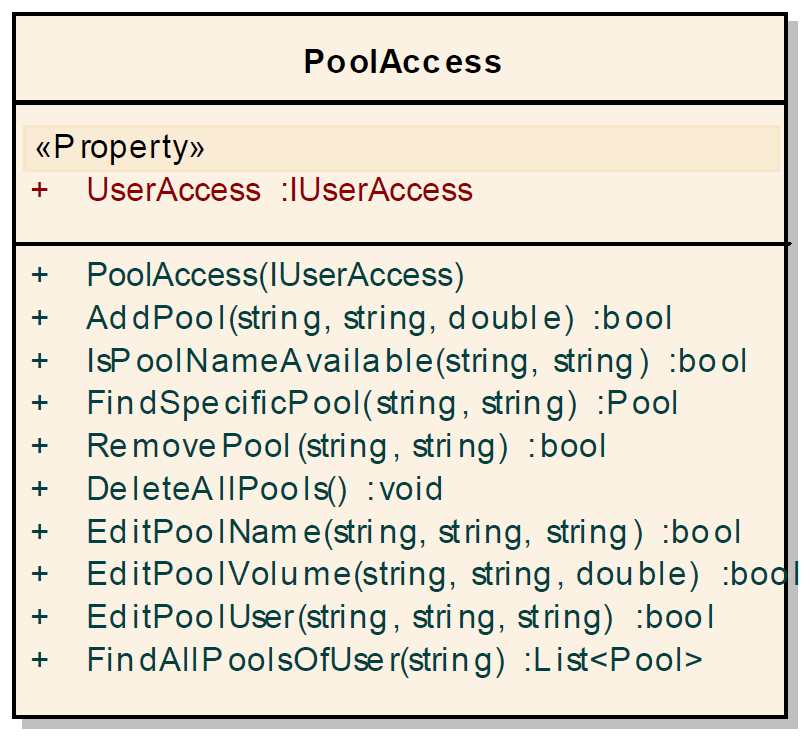
\includegraphics[width=0.46\linewidth]{figs/implementering/poolAccessClass.PNG}
\caption{Klassen PoolAccess.}
\label{fig:poolAccessClass}
\end{figure}

\paragraph{AddPool}%%%%%%%%%%%%%%%%%%%%%%%%%%%%%%%%%%%%%%%%%%%%%%%%%%%%%%%%

\subparagraph{Signatur}
\begin{itemize}
	\item \textit{bool AddPool(string email, string name, double volume)}
\end{itemize}

\subparagraph{Returnere:}
\begin{itemize}
	\item \textit{Boolean}, true hvis poolen er sat ind i databasen uden problemer, ellers false.
\end{itemize}

\subparagraph{Argumenter:}
\begin{enumerate}
	\item \textit{string} email addressen til den bruger som poolen skal tildeles.
	\item \textit{string} navnet som brugeren vil bruge til at identificere poolen.
	\item \textit{string} poolens volume i $m^3$.
\end{enumerate}

\subparagraph{Virkemåde}
\begin{itemize}
	\item Metoden tjekker først om brugeren allerede har oprettet en pool med det sammen navn, hvis dette er tilfældet vil metoden returnere \textit{false}. Metoden sikre også at poolens navn ikke er tomt. Hvis brugeren ikke har en pool med samme navn, vil poolen bliver oprettet i databasen.
\end{itemize}

\paragraph{IsPoolNameAvailable}%%%%%%%%%%%%%%%%%%%%%%%%%%%%%%%%%%%%%%%%%%%%%%%%%%%%%%%%






\subparagraph{Signatur}
\begin{itemize}
	\item \textit{bool IsPoolNameAvailable(string email, string name)}
\end{itemize}

\subparagraph{Returnere:}
\begin{itemize}
	\item \textit{Boolean}, true hvis navnet er ledigt og false hvis det er taget. To brugere kan godt begge have en pool med det samme navn.
\end{itemize}

\subparagraph{Argumenter:}
\begin{enumerate}
	\item \textit{string} email addressen til den bruger som har poolen.
	\item \textit{string} navnet som brugeren har valgt til at identificere poolen.
\end{enumerate}

\subparagraph{Virkemåde}
\begin{itemize}
	\item Metoden finder alle pools i databasen som har dette navn. Derefter tjekker den om en af disse pool tilhører brugeren, ved hjælp af email addressen.
\end{itemize}









\paragraph{FindSpecificPool}%%%%%%%%%%%%%%%%%%%%%%%%%%%%%%%%%%%%%%%%%%%%%%%%%%%%%%%%





\subparagraph{Signatur}
\begin{itemize}
	\item \textit{Pool FindSpecificPool(string email, string name)}
\end{itemize}

\subparagraph{Returnere:}
\begin{itemize}
	\item \textit{Pool} en instans af pool objektet, som har samme attributter som poolen i databasen.
\end{itemize}

\subparagraph{Argumenter:}
\begin{enumerate}
	\item \textit{string} email addressen til den bruger som har poolen.
	\item \textit{string} navnet som brugeren har valgt til at identificere poolen med.
\end{enumerate}

\subparagraph{Virkemåde}
\begin{itemize}
	\item Metoden tjekker først om den valgte kombination af email og navn findes i databasen. Hvis kombinationen findes, henter den poolen og returnere denne.
\end{itemize}








\paragraph{RemovePool}%%%%%%%%%%%%%%%%%%%%%%%%%%%%%%%%%%%%%%%%%%%%%%%%%%%%%%%%

\subparagraph{Signatur}
\begin{itemize}
	\item \textit{bool RemovePool(string email, string name)}
\end{itemize}

\subparagraph{Returnere:}
\begin{itemize}
	\item \textit{Boolean}, true hvis poolen kunne fjernes fra databasen uden problemer, false ved fejl.
\end{itemize}

\subparagraph{Argumenter:}
\begin{enumerate}
	\item \textit{string} email addressen til den bruger som har poolen.
	\item \textit{string} navnet som brugeren har valgt til at identificere poolen med.
\end{enumerate}

\subparagraph{Virkemåde}
\begin{itemize}
	\item Metoden tjekker først om den valgte kombination af email og navn findes i databasen. Hvis kombinationen findes, henter den poolen ved navn og hvis det er brugerens pool bliver den fjernet.
\end{itemize}

\paragraph{DeleteAllPools}%%%%%%%%%%%%%%%%%%%%%%%%%%%%%%%%%%%%%%%%%%%%%%%%%%%%%%%%




\subparagraph{Signatur}
\begin{itemize}
	\item \textit{void DeleteAllPools()}
\end{itemize}

\subparagraph{Returnere:}
\begin{itemize}
	\item \textit{void}.
\end{itemize}

\subparagraph{Argumenter:}
\begin{enumerate}
	\item Tager ikke nogle argumenter.
\end{enumerate}

\subparagraph{Virkemåde}
\begin{itemize}
	\item Metoden er lavet til brug under udvikling og test. Den fjerner alle pools i databasen.
\end{itemize}






\paragraph{EditPoolName}%%%%%%%%%%%%%%%%%%%%%%%%%%%%%%%%%%%%%%%%%%%%%%%%%%%%%%%%





\subparagraph{Signatur}
\begin{itemize}
	\item \textit{bool EditPoolName(string ownerEmail, string currentName, string newName)}
\end{itemize}

\subparagraph{Returnere:}
\begin{itemize}
	\item \textit{Boolean}, true hvis poolen attributter kunne ændres uden fejl, ellers false.
\end{itemize}

\subparagraph{Argumenter:}
\begin{enumerate}
	\item \textit{string} email addressen til den bruger som har poolen.
	\item \textit{string} navnet som brugeren har valgt til at identificere poolen med.
	\item \textit{string} det nye navn som pool skal tildeles.
\end{enumerate}

\subparagraph{Virkemåde}
\begin{itemize}
	\item Metoden tjekker først om det nye navn er gyldigt (ikke en tom string). Så tjekkes det om den valgte kombination af email og navn findes i databasen. Hvis kombinationen findes, henter den poolen ved navn og hvis det er brugerens pool bliver navnet ændret.
\end{itemize}





\paragraph{EditPoolVolume}%%%%%%%%%%%%%%%%%%%%%%%%%%%%%%%%%%%%%%%%%%%%%%%%%%%%%%%%







\subparagraph{Signatur}
\begin{itemize}
	\item \textit{bool EditPoolVolume(string ownerEmail, string name, double newVolume)}
\end{itemize}

\subparagraph{Returnere:}
\begin{itemize}
	\item \textit{Boolean}, true hvis poolen attributter kunne ændres uden fejl, ellers false.
\end{itemize}

\subparagraph{Argumenter:}
\begin{enumerate}
	\item \textit{string} email addressen til den bruger som har poolen.
	\item \textit{string} navnet som brugeren har valgt til at identificere poolen med.
	\item \textit{double} det nye volumen som pool skal tildeles.
\end{enumerate}

\subparagraph{Virkemåde}
\begin{itemize}
	\item Metoden tjekker først om det nye volume er gyldigt (ikke en tom string). Så tjekkes det om den valgte kombination af email og navn findes i databasen. Hvis kombinationen findes, henter den poolen ved navn og hvis det er brugerens pool bliver navnet ændret.
\end{itemize}





\subparagraph{EditPoolUser}%%%%%%%%%%%%%%%%%%%%%%%%%%%%%%%%%%%%%%%%%%%%%%%%%%%%%%%%







\subparagraph{Signatur}
\begin{itemize}
	\item \textit{bool EditPoolUser(string currectOwnerEmail, string name, string newUserEmail)}
\end{itemize}

\subparagraph{Returnere:}
\begin{itemize}
	\item \textit{Boolean}, true hvis poolen kunne fjernes fra tidligere bruger til tilføjes den nye, ellers false.
\end{itemize}

\subparagraph{Argumenter:}
\begin{enumerate}
	\item \textit{string} email addressen til den bruger som har poolen.
	\item \textit{string} navnet som brugeren har valgt til at identificere poolen med.
	\item \textit{string} email addressen til den nye bruger som skal have poolen.
\end{enumerate}

\subparagraph{Virkemåde}
\begin{itemize}
	\item Metoden tjekker først om den valgte kombination af email og navn findes i databasen. Hvis kombinationen findes, testes det om den nye bruger eksistere. Hvis den nye bruger ikke allerede har en pool med samme navn, bliver poolen fjernet fra den gamle bruger og tilføjet den nye.
\end{itemize}






\paragraph{FindAllPoolsOfUser}%%%%%%%%%%%%%%%%%%%%%%%%%%%%%%%%%%%%%%%%%%%%%%%%%%%%%%%%








\subparagraph{Signatur}
\begin{itemize}
	\item \textit{List<Pool> FindAllPoolsOfUser(string ownerEmail}
\end{itemize}

\subparagraph{Returnere:}
\begin{itemize}
	\item \textit{List<Pool>}, som indeholder alle pool tilknyttet en bruger.
\end{itemize}

\subparagraph{Argumenter:}
\begin{enumerate}
	\item \textit{string} email addressen til den bruger, som pools skal findes for.
\end{enumerate}

\subparagraph{Virkemåde}
\begin{itemize}
	\item Først tester metoden om brugeren findes i databasen, hvis denne ikke kan findes smides en \textit{UserNotFoundException()}. Dernæst findes alle pools med tilknytning til brugeren og disse returneres.
\end{itemize}






\paragraph{UserAccess}%%%%%%%%%%%%%%%%%%%%%%%%%%%%%%%%%%%%%%%%%%%%%%%%%%%%%%%%

\textit{IUserAccess UserAccess { get; set; }}